%!TEX root = main.tex
\chapter{Problem Elaboration}
\label{chap:problemelaboration}
\label{problemelaboration}
In this chapter we will elaborate on our problem by defining our task and presenting our high level requirements. We will also introduce GitHub as the choice of version-control system for our implementation.
On the basis of theory, background and related work we will also also present our two main scenarios and the context of these. 

\section{Problem Overview}
\label{problemdefinition}

To answer our research questions we will develop a web-application aimed at software development teams adopting an agile process model. Most agile process models adopt reflection sessions \citep{retrospectivedzone}, and helping users prepare for these sessions in order to gain the best possible learning outcome is one of the main issues our application try to address. Collecting experience related data throughout a working day, allows users to revisit recent(fresh) experiences and trigger reflection upon these experiences. By capturing these daily reflections and storing them for later use allow users to go back to these experiences and recollect the lessons learned. Sharing these notes with the rest of the team allows the team to collaboratively prepare for the retrospective sessions that take place in agile process models. Reviewing these daily reflection notes individually by the user and/or by the team, further helps identify trending issues spanning the iteration and even the whole project over time. The team can also use the shared notes to compare experiences and trigger discussion and reflection upon these. 

Most of these teams use some sort of a version control system with project artifact's, like programming code, text documents etc. We have chosen to focus on GitHub(See section \ref{githubchapter}), but the application could be adapted to work with any version tracker that allows for data collection. \\
Figure \ref{overalltoolprocess} shows the overall process of our application, how user's interact with GitHub and the PeacefulBanana application. 
\begin{figure}[H]
\centering
	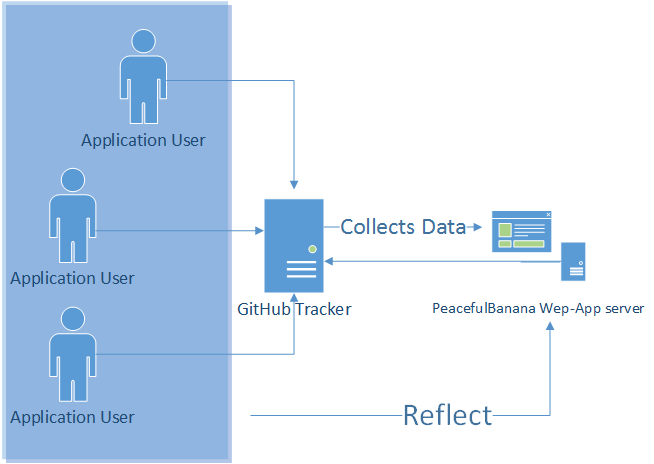
\includegraphics[width=\textwidth]{overalltoolprocess}
\caption{Overall application process}
\label{overalltoolprocess}
\end{figure}

The application will collect relevant data from the project repository on GitHub without any action needed from the user to do so. The application will then \emph{scaffold}, that is present the collected data in a structured frame in order to allow users to revisit and reflect upon agile project experiences, and also share these reflection notes.

The experiences will be presented in several different ways like activity-graphs, mood-graphs and tag clouds. These will act as reflection triggers and help the users to reflect on their work. These experiences will be collected and made available for the users and/or the team later. The application will be designed with reflection in mind, and scenarios was created to demonstrate the most important functionality regarding enhancing reflection in software development teams. Although we evaluate the application in the context of demonstrative scenarios, we see the possibility of the application being used outside of the context provided by scenarios. Users can at any time look into a repository, a milestone or a single issue and the application will provide data that is useful for recollecting experiences and providing a basis for reflection upon these. 

We have worked out two main scenarios, which can be seen in Section \ref{sec:scenarios}. Evaluation of the application will be conducted in the context of these in order to gain feedback on how the application may answer our research questions. Evaluation will be a usability test, an expert review and a focus group. 

\section{Github}
\label{githubchapter}
This section will introduce GitHub, the features GitHub provides and the rationale behind choosing GitHub as the VCS for our application implementation. 
GitHub is a web-based hosting service for software development projects that use the Git revision control system\citep{git,github}. GitHub offers both paid plans for private repositories, and free accounts for open source projects.

GitHub provides users with integrated issue tracking, code review, project wiki, useful statistics and more. 
Motivational points for choosing GitHub as the revision control system to integrate with are several. Some technical aspects are that GitHub provides developers with a simple to use API\citep{githubapi}, with libraries for integration with most of the commonly used programming languages, like Java\citep{jgit}.
In addition to the technical aspects, GitHub is the most used revision control system ,as of January 2013 GitHub announced it had passed the 3 million users mark and now hosting more than 5 million repositories and is a application many in our evaluation group already use in their development projects\citep{githubnumbers}.

\subsection{Authentication}
In order to retrieve data from repositories on GitHub, GitHub users need to allow the specific application access to their repository. This is done by authentication, which is a feature offered from GitHub to external applications through their GitHub APIv3\footnote{http://developer.github.com/v3/}. 
\subsection{Repositories}
GitHub is a repository hosting service for software development projects. A repository contains all the project files, may it be code, images, and other documentation. This means that all content in a project is connected to this repository. In addition to documentation and file content, GitHub provides integrated issue tracking, which is connected to this repository and could also be connected to one or several milestones. 
\subsection{Commits}
Say some of your project files have been changed, for example some code snippet in a Java file. The way to save these changes to your local branch is by commits. A commit can consist of code line additions, deletions, files added, changed or removed. When you are ready to save the changes, you commit them in a command line together with a commit message which is a short text describing the changes you have done. \\
When a user is ready to push one or more local commits to the project repository, it can be done via the command git push in the command line. It is now the HEAD revision and the new code and commits can be seen on the GitHub page.
\subsection{Milestones and Issues}
\begin{quote}
\em GitHub Issues can be assigned to a user to make it easy to know who's working on what, or which issues you need to tackle next.
\end{quote}
\begin{figure}[H]
\centering
	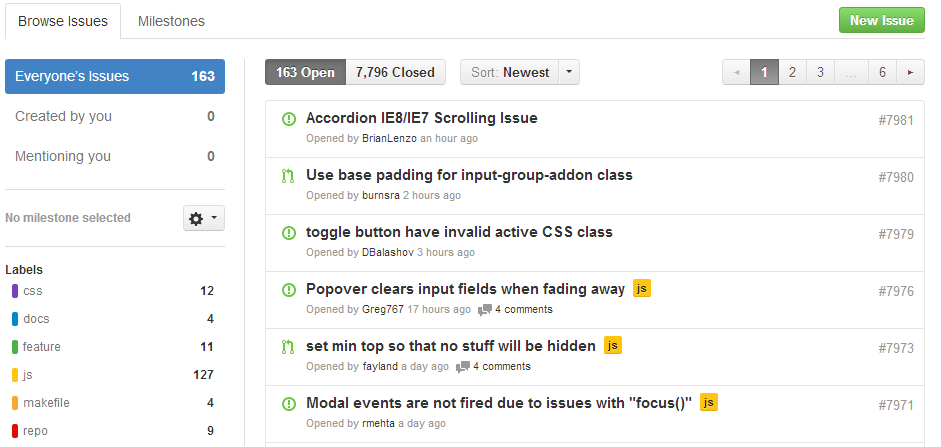
\includegraphics[width=\textwidth]{githubissuetracker}
\caption{Example of GitHub's issue tracker overview. This particular example is from Twitter Bootstrap's current issue tracker}
\label{githubissuetracker}
\end{figure}

Every GitHub repository has an issue tracker, that allows users to track bugs and focus on features. An example of such an issue tracker can be seen in Figure \ref{githubissuetracker}, which depicts the current issue tracker of Twitter Bootstrap's public repository\footnote{\url{https://github.com/twitter/bootstrap/issues}}. Milestones and issues help manage large projects, where issues especially makes for a great TODO list, similar to a product backlog. Only {\bf collaborators} can create and view issues on private repositories. On public repositories anyone can create and view issues. 
\begin{itemize}
\item GitHub issues can be assigned to a user, which makes it easy to know who's working on what, or which issues should be handled next. Milestones are a good way of helping team members to work towards a goal. A team can set a due date, name a milestone and then start assigning issues to that milestone. An example of a Milestone could be a due date of a project demo or delivery. Any number of issues can then be assigned to this milestone, and thus be connected to it. 
\item Issues know all about commits. GitHub enables referencing and closing issues with Commit Messages. By using a few simple keywords you can close an issue right from a commit message, or just leave a note on the issue.The syntax to do this is as follows: To close issue \#35 , a commit message containing 'closes \#35' , will close issue number 35 when pushed to GitHub. Other keywords are: close, closes, closed, fixes, fixed. 

To leave a note on issues can be done by simply mentioning the issue number without any keywords in a commit message. F.ex "This commit references \#35". Anyone with write access to a repository may close an issue or leave a note.
\end{itemize}

\section{Using technology to promote learning from reflection}
The world wide web and modern technologies provides easy access to enormous amounts of information. This means that in order to learn, learners must be able to make sense of the information collected.  
In order to achieve this and make conscious decisions of how to use information, learners need to reflect on the information they collect. Reflection upon the process of solving problems is necessary to achieve a good result and to improve the ability to learn from experiences. When supporting learning with technology, this technology should promote these aspects within learning\citep{Lin1999}. 

By implementing this proof of concept application, we wish to provide technology that enables efficient information retrieval, and to provide scaffolds or structured frames that support reflective thinking and problem solving. In our development of PeacefulBanana this means utilizing both individual and collaborative learning experiences. 

\subsection{Agile Retrospective}
The agile retrospective is held at the end of an iteration in order to learn from the iteration and not repeat mistakes. A model of how a retrospective can be done is shown in \citep{Derby2006}. The purpose is to learn what works and what does not work, and make the adjustments necessary for the next iteration. This way the team makes sure that every iteration introduces some improvements in the team's process. There are two fundamental questions the retrospective is intended to answer:
\begin{itemize}
\item What went well during the last iteration that we continue doing?
\item What could we do differently in order to improve?
\end{itemize}
These questions are something we incorporated into both the individual and collaboration parts of the PeacefulBanana application, since they are a vital part of the learning outcomes in agile retrospectives. The application primarily aims at providing a structured frame for the retrospective, although all parts of the retrospective needs to be considered during development. \\
Figure \ref{fig:itcyclemodel} shows where the retrospective fits in the overall agile iteration cycle, and the table in Figure \ref{fig:retrospectivetable} shows the retrospective process in more details \citep{Derby2006}.
Knowing the process of the agile retrospective was important during development. The PeacefulBanana application provides teams with a frame for the retrospective, containing the most relevant issues the team should discuss. This fits with the \emph{Set the stage} phase in Figure \ref{fig:retrospectivetable}. This frame also brings the team a shared and collaborative setting, since it contains the most commonly worked on issues for the whole team. This covers the \emph{Gather Data} and \emph{Generate Insights} phase. Additionally user's can use the application to prepare individually for the retrospective. Having these individual points of view may give the team greater insight to issues that may have been lost in the collaborative setting. I.e.if a user's work differs a lot from the rest of the team, this may indicate missing competence-overlap and needs to be discussed. \\
The application provides the team with a printable template or frame they can follow during the retrospective session, which they can use to write down their thoughts on each of the issues the team discuss. Since a vital part of the retrospective session is to write down the learning outcomes, the printable frame allows the team to collect this, covering the last two phases in a retrospective. Since the retrospective session is conducted analogically, these answers are written down on paper, and is not collected by the system. 
\begin{figure}[!htpb]
\centering
	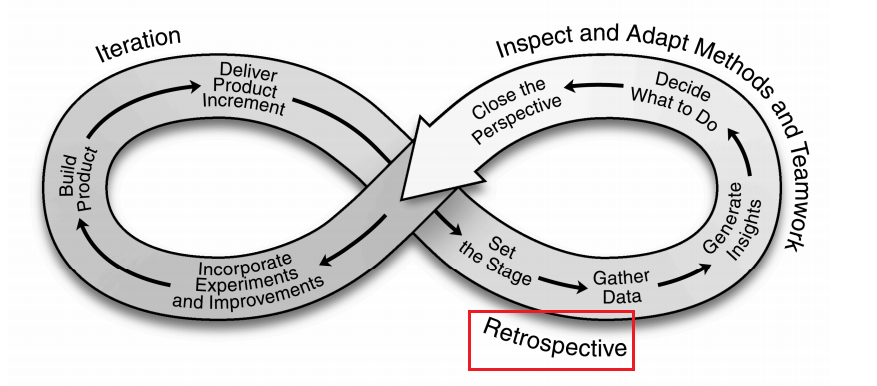
\includegraphics[width=\textwidth, keepaspectratio=true]{iterationcyclemodel}
\caption{Retrospectives in the agile iteration cycle \citep{Derby2006}}
\label{fig:itcyclemodel}
\end{figure}
\begin{figure}[!htpb]
\centering
	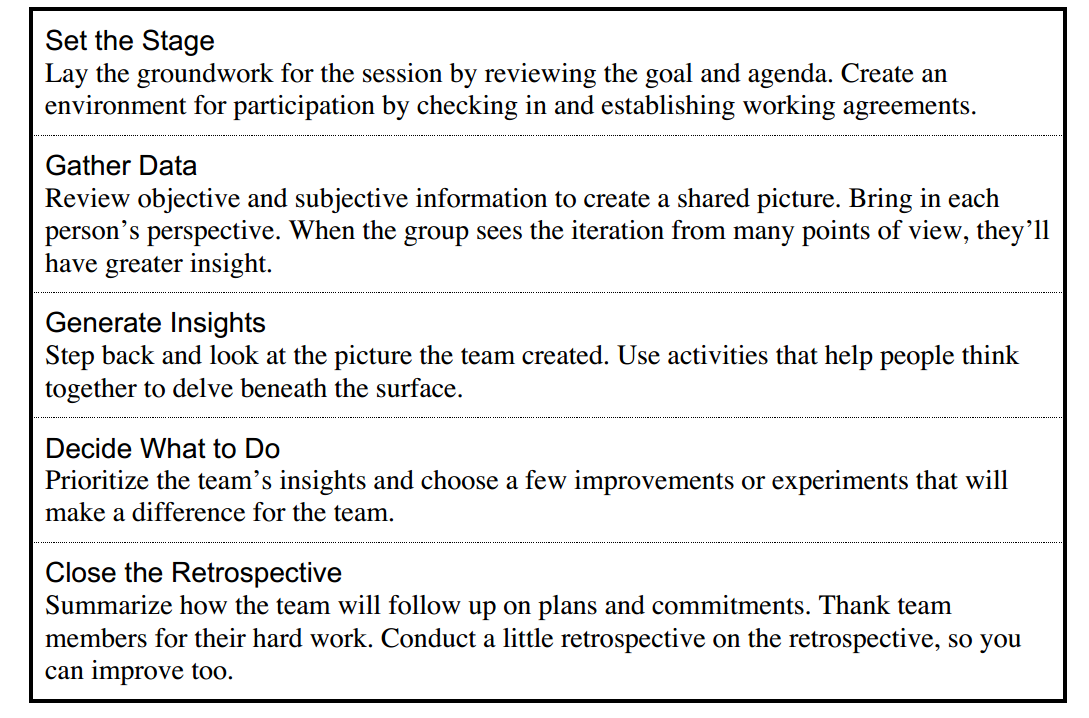
\includegraphics[width=\textwidth, keepaspectratio=true]{retrospectivetable}
\caption{Agile retrospectives - from beginning to end \citep{Derby2006}}
\label{fig:retrospectivetable}
\end{figure}

\section{Scenarios}
\label{sec:scenarios}
Based on related work, we have developed two scenarios to show what we want our application to support in terms of collaborative learning from reflection. These two scenarios will provide a basis for the requirement elaboration and design choices in development of the tool. 
The application is developed to be used by agile software development teams in a real working environment. Further we developed the application with teams using GitHub as a version-control system in mind. During the project work the team will use GitHub to collect information. The PeacefulBanana application can then be used to gather this information and present it in a scaffolded, or structured way, mainly to enable user to trigger reflection individually and to used in retrospective sessions. Users can though, at any time go into the application and gather relevant data if they want to. This data will help the team see trending issues and problems they have come upon in the process. Each member of the group will register as a user on the PeacefulBanana application and the users will then be connected together as a team, if they are part of the same team on GitHub. 

The two scenarios described in the next sections provides a demonstration of how we envision the usage of the PeacefulBanana application in the context of different settings. First as a individual application on a daily basis, then as part of a team collaborative reflection session.
These two scenarios were developed early in the development process. The first scenario features using the application at the end of each working day as inspired by the 5-minute daily reflection(See Section \ref{whatdoesitdo}). The second scenario is set in the context of that in each iteration there is a retrospective reflection session at the end. 

\subsection{Scenario 1 - Individual use on a daily basis}
\label{scenario1}
In this scenario, our team users will be using the application on a daily basis at the end of each working day.
When users enter the web-application, they will get a notification with a prompt to do the daily status update.

\begin{figure}[h!]
\label{newnotification}
\centering
	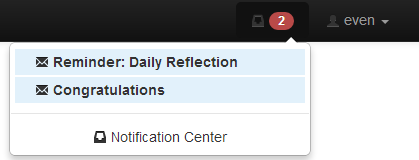
\includegraphics[width=\textwidth]{newnotification}
\caption{The user has clicked the notification icon and can see his new notifications}
\end{figure}

  When clicking the notification, the user is presented with a summary of their individual activity in the last 24 hours.
  This summary compares the commit activity of the user with the team's, and also presents a tag cloud representing the trending issues of the last day. The user is then prompted to input todays mood, their top two contributions \emph{"What did I do good?"} , and their top 2 points to improve on \emph{"What could I do better?"}. Finally the user can submit the form and choose to share these experiences with the team for collaborative use. The daily reflection notes are saved and can be reviewed at any time, and also shared any time by the user. The idea is that the application will be used to revisit todays experiences with collected information presented in a way that triggers reflection upon these experiences. Information is collected and inspire new experiences. After working on a project that day, users "step back" to reflect on what happened during the day, and on the experiences they encountered. The application provides scaffolded data to further trigger this reflection process. This process consist of returning to the experiences of that day, re-visit the experiences and attend to the feelings, like inputing todays mood. This reflection will help users to derive their top two improvements and contributions of the day\citep{Krogstie2011}. The application thus captures the experiences and reflections made by the user and allows for re-visiting of these at a later date by storing them in the system. 

\subsection{Scenario 2 - Team use after each iteration}
\label{scenario2}
In this scenario, users will be using the application as part of the preparation for the agile retrospective sessions. As a requirement users need to use the application as described in Scenario 1(section \ref{scenario1}). This means going through the daily reflection note process each day they have contributed to a project. Based on the notion that iterations in agile teams often last for 30 days or less\citep{scrumguide}, the scenario was created with the aspect of iterations lasting at least two weeks each. This way enough data can be gathered through the reflection notes, and experiences are still fresh. \\
Users will individually be able to prepare for these retrospective sessions, while the team can use the application collaboratively as preparation for the session as well.
Users will in this scenario use the application to indicate how the project has been progressing over the last iteration, tightly coupled with one or several milestones. They will be able to generate tag clouds based on the trending issues in the relevant milestones, activity graphs and mood trajectories. Examples of such a tag-cloud and mood-graph can be seen in Figure \ref{tagcloudfuncscenario} and Figure \ref{moodgraphscenario}. Also if the users have chosen to share any of the individual reflection notes from scenario 1, these will be visible and can be used by the team as a whole to draw conclusions from the previous iteration, create a discussion and make comparisons. The application will enable the team to see the whole iteration more clearly, but also enable teams to dive into certain issues or milestones that showed to be of particular interest, and thus create a discussion around the experiences made by the team members. 
\begin{figure} 
\centering
	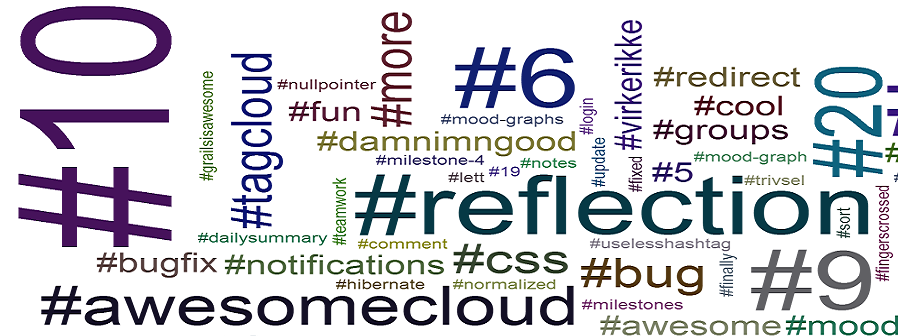
\includegraphics[width=\textwidth]{tagcloudfunc2}
\caption{Example of a team tag-cloud.}
\label{tagcloudfuncscenario}
\end{figure}
\begin{figure}[H]
\centering
	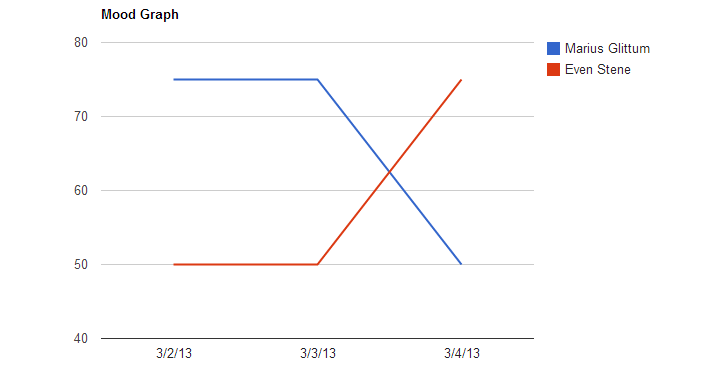
\includegraphics[width=\textwidth]{moodgraph}
\caption{Example of a team mood-graph over a period of time.}
\label{moodgraphscenario}
\end{figure}
As a final part of the scenario, teams will be able to create a \emph{workshop} based on any previous iteration period. When the workshop has been created, the team manager or the team as a whole get a set of system generated questions that relate to the workshop iteration. These data are gathered from the team's reflection notes and general GitHub data, and try to present what issues the team have been working the most on for the iteration. The team will, after selecting the questions or topics they want to discuss in the retrospective session, be able to print these as a guide the team can follow during the session. Their reflection outcomes or lessons learned can be noted on the paper by each team member, together with thoughts or comments.